\chapter{Introdução}
\label{cap-introducao}

A gestão dos ativos (Asset Management) de uma organização seja ela pública ou privada, independente de sua finalidade, é cada vez mais adotada ao redor do mundo como uma ferramenta para enfrentar os desafios econômicos impostos por um mercado globalizado diversificado ou uma sociedade que exige do poder público maior transparência e eficiência no emprego de seus tributos, já que a administração eficiente dos ativos tem a capacidade de aperfeiçoar o desempenho técnico e econômico dos equipamentos, acelerar o retorno sobre os investimentos realizados, e colaborar com planejamento organizacional trazendo previsibilidade e controle dos gastos envolvidos. 

Dentre as áreas da gestão de ativo, a manutenção é geralmente encarada como uma despesa que se deseja ao máximo adiar, não sendo uma prática suficientemente valorizada. Esta opinião é compartilhada, devido ser a manutenção uma fonte de custo, que não acrescenta um valor perceptível ao cliente final do produto ou serviço prestado pela organização, e gera indisponibilidades momentâneas no uso de bens e recursos.
Todavia, inevitavelmente a ação do tempo e o uso fazem com que equipamentos e instalações se desgastem, e precisem periodicamente de reparos, regulagens e limpeza para continuarem operando eficientemente.

A necessidade de se ter uma gestão de manutenção efetiva está se tornando cada vez mais importante, isso porque  reduzir desperdícios e executar com eficiência os processos de uma organização, tem se tornado cada dia mais necessário. Sendo o maior fator que impulsiona decisões hoje, o custo e o lucro, quanto se está gastando para produzir e quanto se está obtendo de lucro. É aí que a manutenção se faz importante, porque o custo de realizar uma manutenção regular pode se tornar muito pequeno quando comparado ao custo de uma interrupção na produção ou atividades suportadas por ativos que necessitem de manutenção.

Assim, pode se definir com sendo um dos principais propósitos da manutenção, assegurar que todos os equipamentos requeridos para produção estejam funcionando com 100\% de eficência o tempo todo, por meio de inspeções diárias e pequenos ajustes, os quais ajudarão na detecção de problemas menores, diminuindo a chance de esses problemas se tornarem maiores ou até incorrigíveis. Krar \cite{krar2009} ainda diz que para se atingir uma manutenção regular e efetiva, é preciso que haja participação de todos, desde o alto executivo até as pessoas do operacional.



Com o reconhecimento da importância de se empregar processos efetivos de manutenção nas organizações, surgiu nos anos setenta, Associações de Manutenção, na Espanha, México e Portugal, que despertou o interesse em profissionais brasileiros pelos conceitos, métodos e tecnologias que essa área dispõe. Em 1938, no III Congresso Ibero-Americano de Manutenção, foi aprovada a proposta de uma entidade no Brasil. Foi fundada então, em 17 de outubro de 1984, a Associação Brasileira de Manutenção, mudando seu nome em 2012 para Associação Brasileira de Manutenção e Gestão de Ativos. No começo, a ABRAMAN só tinha representantes dos setores de petróleo, eletrecidade, siderugia e transportes. Mais tarde a associação ganhou aderência por parte de setores diversos, por exemplo, hoje em dia a ABRAMAN emite certificados MBA de gestão de ativos para Instituições de Ensino Superior, assim como para outros setores. 

Em 1983, o IBP (Instituto Brasileiro de Petróleo) criou um documento nacional para análise da situação da manutenção no Brasil, a responsibilidade da elaboração passou para ABRAMAN desde a criação da associação em 1984, que em 1993, aderiu aos moldes de apresentação e desenvolvimen da AEM (Associação Espanhola de Manutenção), o qual é mantido até os dias de hoje.  

O Documento Nacional - A Situação da Manutenção no Brasil, apresenta resultados de pesquisas realizadas bienalmente, desde 1985, com indicadores de performance da Manutenção e Gestão de Ativos, presentes nos principais setores de produtos e serviços que movimentam a economia brasileira. No site da ABRAMAN \cite{abraman}, onde constam essas informações, também relata que um dos insumos para o documento são pesquisas e levantamento de índices em áreas de enfoque como \emph{Forma de Atuação, Nível Hierárquico, Pessoal Próprio, Quadro Técnico, Rotatividade e Contratação de Pessoal, Contratação e Conceito dos Serviços, Critérios na Contratação, Composição dos Custos, Aplicação dos Recursos - Pessoal, Qualidade na Manutenção, Custo por Faturamento, Disponibilidade Operacional, Idade Média, Valor de Estoque e Segurança Industrial}. O documento tem uma alta relevância por representar de forma detalhada uma análise da situação da função no Brasil. Tendo servido como fonte de dados para profissionais, estudantes, pesquisadores e gerentes de empresas.

Em uma de suas últimas pesquisas, no ano de 2013, a ABRAMAN revelou que o custo total da manutenção representou em média 4,69 porcento do faturamento bruto nas empresas brasileiras, perfazendo uma parcela significativa do PIB nacional, na verdade o valor mais alto dessa estatística desde o inicio da série histórica, iniciada em 1995, conforme mostra a Figura~\ref{custo_anual_2013}.

\graphicspath{{figuras/}}
\begin{figure}[h]
\centering
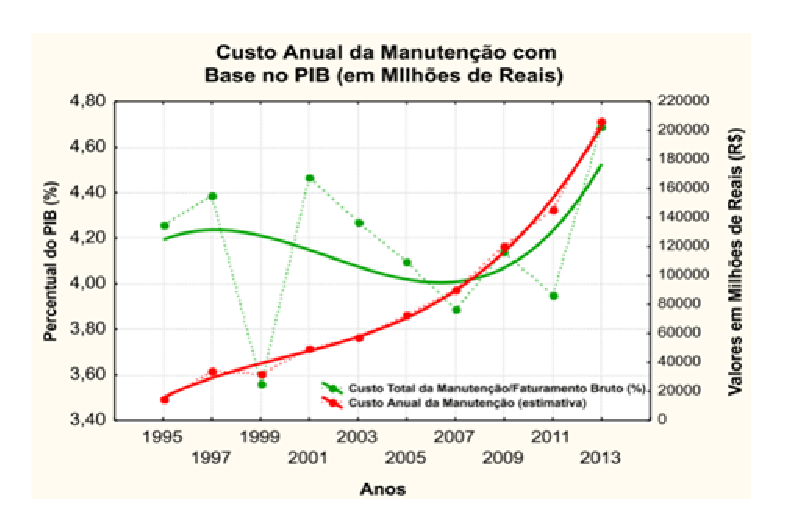
\includegraphics[width=0.8\textwidth]{dados_pib_pesquisa_intro.eps}
\caption{Custo anual da manutenção com base no PIB. \textbf{Fonte: ABRAMAN, Documento Nacional 2013.}}
\label{custo_anual_2013}
\end{figure}


Isto esta aliado ao que afirma DEKKER \cite{dekker1998}, que relata que os gastos com manutenção tendem a crescer em todos os setores da economia, a despeito do desenvolvimento tecnológico, o que provocaria pensar que é uma contradição, porém as principais causas são a contínua expansão dos bens de capital e as exigências de mercado que impõe uma alta taxa de disponibilidade e confiabilidade dos equipamentos.

Dado essas informações, considerar a manutenção somente uma atividade operacional, é não enxergar o valor significativo envolvido nessa área, nem sua responsabilidade para com a qualidade e imagem da organização. A função da manutenção deve possuir políticas e estratégias para que ela tenha a mesma relevância que outras funções da organização, atribuindo-lhe diretrizes e metas.	

No setor público, as políticas de gestão da manutenção, como a de muitas outras áreas, tendem a evoluir em menor velocidade que na iniciativa privada, devido suas características legais e burocráticas que apesar de necessárias, para combater as práticas patrimonialistas, acabam por dificultar a inovação gerencial. Contudo o Estado precisa de um modelo de administração que traga resultados efetivos gastando a menor quantidade de recursos possíveis.


Neste contexto se insere o objeto de estudo deste trabalho: A Universidade de Brasília – UnB. A qual segundo rankings nacionais, como o ENADE/MEC, e internacionais, como o \emph{Britanico Quacquarelli Symonds} (QS), se encontra entre as melhores do país e da América Latina, 10º e 9º lugar respectivamente. A Universidade possui grande importância por sua localização geográfica, capital do Brasil, e pesquisas desenvolvidas em diversas áreas de conhecimento, incluindo Engenharia e Saúde. Algumas destas pesquisas são realizadas em parceria com as melhores universidades do mundo, e induzem o denvolvimento do país, como por exemplo, a estação de monitoramento e correção diferenciada, que integra o \emph{Global Navigation Satellite System} (Glonass), em parceria com a Rússia, e as pesquisas na área da robótica desenvolvidas pelos departamentos de Engenharia de Software e Eletrônica da Universidade.

A UnB detém diversos laboratórios de pesquisa e certificação de alto valor e tecnologia, com um grande número de aparelhos e equipamentos científicos com sistemas complexos, todavia como outras instituições públicas de ensino superior, adotou políticas para a aquisição de um parque cientifico e tecnológico sem pensar em aspectos importantes para a manutenção, o que atrapalha os procedimentos em caso de defeitos, cometendo erro de não verificar a existência de meios humanos e materiais para a manutenção dos equipamentos, além disso, dispõe de processos de gestão de manutenções pouco informatizados, não possuindo indicadores de desempenhos claros que auxiliem seus gestores a tomada de decisão. Segundo \cite{limacastilho2006} isso reflete, no caso particular da Universidade de Brasília, numa taxa de indisponibilidade exagerada dos equipamentos e instalações importantes para os laboratórios de ensino, pesquisa e de apoio administrativo, tendo como conseqüência a diminuição da capacidade produtiva da instituição e a insatisfação daqueles que dependem desse serviço.

Assim, a confiança nos serviços oferecidos pela Diretoria de Manutenção de Equipamentos – DIMEQ, unidade responsável por prover a manutenção e o reparo de equipamentos da Universidade, fica comprometida. 

Portanto, este trabalho tem como escopo fornecer fundamentos e indicadores de desempenho que auxiliem na gestão da manutenção dos equipamentos da Universidade, mais precisamente dos equipamentos eletrônicos. Estes são de maneira geral aqueles que possuem na maioria dos seus circuitos, componentes eletrônicos, tais como: Equipamentos biomédicos e de análise clínica, de laboratório, de som e de imagem, e aqueles que promovem a infra-estrutura de rede e comunicação. Cita-se como exemplo: Os monitores de vídeo para microcomputadores, equipamentos de som e projetores de multimídia, balanças eletrônicas, suítes, roteadores e outros.

Entende-se por gestão \lq\lq gerenciar é previnir e planejar, comandar, coordenar e controlar \rq\rq, Henry Fayol dá essa definição no livro General and Industrial Manegement, 1949, e \cite{prasadgulshan2011} diz que ela passa as funções do gerenciamento para se alcançar os resultados desejados. Gerenciar leva você a atingir suas metas, é necessário defini-lás para saber se aquilo que se quer gerir está gerando os resultados esperados, assim como trazer melhorias.

A manutenção, melhor definida no Capítulo~\ref{cap-manutencao}, é aplicar técnicas para manter ou restaurar um ativo para um estado ao qual ele possa realizar as funções requeridas. Gestão da manutenção seria então, controlar, planejar, coordenar a aplicação dessas técnicas para que se possa ter esses ativos gerando resultados positivos e de acordo com o esperado.

Dessa forma, procura-se encontrar nesse trabalho fundamentos para que se possa implementar um gestão da manutenção eficiente na UnB. De acordo com trabalho de \cite{limacastilho2006} que descreve como o DIMEQ funcionava em 2006, ele possui um software, o SIPAT - Sistema de Informações Patrimoniais, que tem como principais funções registrar \emph{acompanhamento do equipamento no período de garantia, cadastro, histórico de manutenção ou procedimento da manutenção e atualização de dados técnicos}. Essas funcionalidades não te dão uma previsão de falhas do equipamento, a criticidade de se ter o equipamento parado por causa da manutenção, o custo de se ter esse equipamento parado e a consequência de sua ausência nas atividades que ele suporta.

O trabalho busca fornecer uma solução informatizada a qual, por meio de indicadores, possa prever quando o equipamento irá falhar, para saber quando realizar a manutenção, os tipos de manutenção que podem ser aplicadas a um certo tipo de equipamento, aquela que possa ser mais eficiente, e assim a partir dos custos de cada opção, auxiliar o gestor na melhor decisão, se é continuar realizando manutenções em um determinado equipamento ou se é melhor considerar a sua substituição. Serão utilizados na solução conceitos como Tempo Médio de Falha, Tempo Médio de Reparo, Tempo Médio Entre Falhas, disponibilidade, confiabilidade e custo. 


%------------------------------------------------------------------------------%

\section{Problema}

Como melhorar a gestão da manutenção de equipamentos eletrônicos na UnB, por meio do desenho de uma solução que informatize-a, e apresente indicadores de desenpenho que auxilie seus gestores na tomada de decisões quanto ao tipo de manutenção que será aplicada a esses equipamentos ou quanto a substuição dele, levando em consideração o custo da escolha. 

%------------------------------------------------------------------------------%

\section{Justificativa}

O trabalho propõe melhorar a gestão da manutenção da UnB, tendo em vista que a má gestão da manutenção desperdiça recursos, trazendo gastos extras e não planejados, e também gera soluções precárias e tardias que elevam a taxa de indisponibilidade dos ativos, como os equipamentos eletroeletrônicos e hospitalares. Além do que a má gestão pode diminuir o tempo de vida útil dos equipamentos tendo no caso particular da UnB, a consequência da diminuição da produção cientifica e da qualidade de ensino.

Em contrapartida, uma melhor gestão da manutenção maximiza a disponibilidade, confiabilidade e segurança dos equipamentos. O que traz maior previsibilidade dos custos, saindo da cultura do \lq\lq quebrou-concerta\rq\rq, atuando-se preventivamente. As falhas inesperadas diminuem fazendo com que o setor de manutenção contribua com o sucesso do negócio e não seja apenas um setor secundário ou de apoio, seja um setor consolidado que contribua ativamente com a melhoria da Universidade.



%------------------------------------------------------------------------------%

\section{Objetivo Geral}
 
O objetivo geral deste trabalho consiste na proposta de uma solução que informatize a gestão da manutenção de equipamentos eletrônicos da UnB, por meio da análise do seu ciclo de vida e da criação de modelos de manutenção, como os mostrados na Seção~\ref{sec_modelos_manutencao}, que possam melhor atender as necessidades de um certo tipo de equipamento. Assim como a realização de um estudao de caso, para validação da solução proposta. 

O estudo de caso consistirá na análise da recente decisão de se substituir o uso de projetores por televisões nas salas de aula da FGA, analisando as características de cada equipamento, seu ciclo de vida, confiabilidade, desempenho e custo.


%------------------------------------------------------------------------------%

\section{Objetivos Específicos}

Os objetivos específicos do trabalho são:

\begin{enumerate}
	\item Identificar falhas na gestão da manutenção de equipamentos eletrônicos da UnB, para sugerir melhorias, voltadas principalmente para a análise do ciclo de vida dos produtos.
	\item Sugerir uma solução que informatize dados importantes para a manutenção da Universidade, e forneça indicadores que auxiliem seus gestores na tomada de decisões.
	\item Simular a aplicação dos indicadores da manutenção por meio de um software interativo de cálculo numérico (MATLAB) 
	\item Validar solução por meio de um estudo de caso.
	\item Apresentar e descrever normas que padronizem a manutenção e gestão de ativos.
\end{enumerate}

%

\chapter{Metodologia}

Esta etapa da pesquisa aborda o objeto de estudo deste trabalho – a gestão das manutenções de Equipamentos Eletrônicos pela Universidade de Brasília, com vistas a conhecer como está estruturada a Diretoria da Manutenção de Equipamentos DIMEQ/UNB e como se dá a operacionalização destas manutenções, por meio de estudos descritivos do organograma da instituição Universidade de Brasília e entrevistas realizadas com os setores da DIMEQ.

Foi realizada uma extensa revisão bibliográfica que é parte de uma pesquisa exploratória, para se obter conhecimento sobre conceitos relativos ao tema, como manutenção, tipos de manutenção, modelos no Capítulo~\ref{cap-manutencao}, bem como gestão de ativos, ativos, sistema de gestão de ativos e normas relacionadas apresentados no Capítulo~\ref{cap-ativos}, softwares de gestão da manutenção Capítulo~\ref{cmms} e medidas básicas de tolerância a falhas, como  Tempo Médio de Falha, Tempo Médio de Reparo, Tempo Médio Entre Falhas, disponibilidade, confiabilidade e custo encontrados no Capítulo~\ref{falhas}.

Assim como a realização de entrevistas para obtenção de informações sobre como são realizadas as manutenções dos equipamentos eletrônicos, quem são os envolvidos, as ferramentas de gestão utilizadas e outras características existentes no processo realizado pelo DIMEQ/UNB.

Foi então comparado o que diz a literatura, para detectar possíveis fragilidades no processo, ao tempo de propor mudanças para informatização do processo e a criação de indicadores de desempenho da manutenção, pela abordagem quantitativa, que é feita por meio de registros e análises dos dados coletados dos equipamentos escolhidos para o estudo. O estudo de caso teve sua realização com base na recente decisão de se trocar os projetores por televisões nas salas de aula da UnB-FGA. 

\section{Descrição da Diretoria de Manutenção de Equipamentos (DIMEQ)}

Em 30 de outubro de 1987, pelo ato da reitoria nº 550, foi criada Diretoria de Manutenção de Equipamentos - DIMEQ, anteriormente denominado Centro de Manutenção de Equipamentos Científicos – CME, da Fundação Universidade de Brasília, garantido a ela desde então o tratamento autônomo e descentralizado sob o aspecto orçamentário, financeiro, administrativo e gerencial \cite{dimeq}.

Por este ato da reitoria foi atribuída a DIMEQ à responsabilidade de promover, com qualidade, a manutenção e o reparo nos equipamentos da Universidade, introduzindo novos conceitos metodológicos e técnicos para que sejam reduzidas as paradas de funcionamento desses equipamentos; visando a redução de custos, a satisfação do usuário e a viabilização das atividades de ensino e pesquisa.

Na estrutura organizacional da DIMEQ estão compreendidas quatro seções especializadas, a saber, Seção de Apoio a Logística, Seção de Eletrônica e Informática, Seção de Eletromecânica e Seção Mecânica. Esta configuração se fez necessária, em suma, pelos tipos de equipamentos que a Universidade possui, os quais precisam ser agrupados, pois cada tipo de equipamento necessita de uma mão de obra especifica, bem como instrumentos e ferramentas para fins de manutenção. São eles, equipamentos eletrônicos, de informática, eletromecânicos, eletrotécnicos, ópticos e de mecânica fina, e os mecânicos que, por sua vez, se dividem de refrigeração e de mecânica geral.

Os serviços prestados pela DIMEQ devem atender uma comunidade acadêmica bastante ampla, o que faz do processo de manutenção permanente um grande desafio, sendo composta, segundo informações do Anuário Estatístico da UnB 2015 \cite{anuario2015}), de 2.695 professores, 2.623 técnicos-administrativos e 36.372 alunos regulares e 7.576 de pós-graduação. Constituída por 26 institutos e faculdades e 21 centros de pesquisa especializados, oferecendo 109 cursos de graduação, e 147 cursos de pós-graduação stricto sensu e 22 especializações lato sensu. Os cursos estão divididos em quatro campi espalhados pelo Distrito Federal: Darcy Ribeiro (Plano Piloto), Planaltina, Ceilândia e Gama, possuindo diversos órgãos de apoio como o Hospital Universitário, a Biblioteca Central, o Hospital veterinário e a Fazenda Água Limpa.

Somado a grande comunidade acadêmica que a DIMEQ precisa atender, encontra-se o diversificado parque científico que a Universidade de Brasília possui. Esta diversificação, a complexidade e quantidade de equipamentos demandam, segundo \cite{limacastilho2006} um elevado estoque de peças de reposição, espaço físico, qualificação permanente dos técnicos, meios de transporte específicos e, sobretudo, um sistema de gerenciamento e comunicação que esteja em constante evolução, pronto a atender as necessidades emergentes. Há ainda, diversos equipamentos importados que requerem na maioria das vezes, serviços especializados.

Ao se visualizar os números da Universidade, pode se ter uma noção do desafio que é gerenciar as manutenções dos equipamentos, ainda mais quando se estuda o crescimento da população Universitária da UNB de 2006 a 2014, conforme demonstra os Figura~\ref{grafico_dimeq1} e Figura~\ref{grafico_dimeq2}, retirados do anuário estatístico da Universidades de 2011 e 2015, respectivamente. Eles revelam que nestes 8 anos a população universitária cresceu 56,95\% aproximadamente.

\graphicspath{{figuras/}}
\begin{figure}[h]
\centering
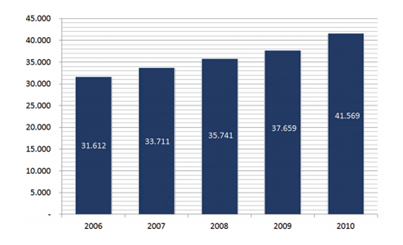
\includegraphics[width=0.9\textwidth]{grafico_dimeq1}
\caption{Evolução da população universitária da UnB, 2006 a 2010. \textbf{Fonte: Anuário estatístico da Universidade de Brasília, 2011.}}
\label{grafico_dimeq1}
\end{figure}


\graphicspath{{figuras/}}
\begin{figure}[h]
\centering
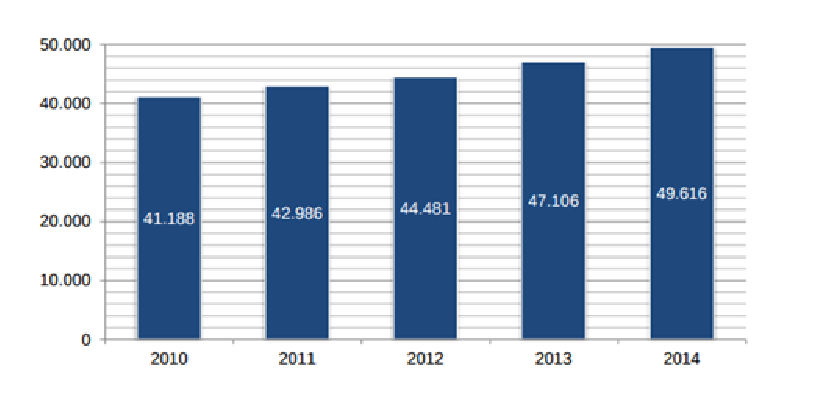
\includegraphics[width=0.9\textwidth]{grafico_dimeq2.eps}
\caption{Evolução da população universitária da UnB, de 2010 a 2014. \textbf{Fonte: Novo anuário estatístico da Universidade de Brasília, 2015.}}
\label{grafico_dimeq2}
\end{figure}

Todo esse crescimento deve ser levado em conta ao se analisar o serviço de Manutenção oferecido pela DIMEQ, pois sua conseqüência é um enorme descompasso entre a quantidade de adquiridos e os recursos aplicados na preservação desse patrimônio. Além de que, conforme relata \cite{limacastilho2006} ao se adquirir esses equipamentos \lq\lq patrimônios\rq\rq a DIMEQ não foi ouvida cometendo assim um erro conceitual grave para gestão da Manutenção, como já foi relatado no capítulo de Manutenção do presente trabalho.
	
O gerenciamento da manutenção do parque cientifico da UnB é informatizado, permitindo a todos os usuários solicitar e acompanhar reparos nos equipamentos ou a programação de manutenção preventiva de todos os equipamentos cadastrados no Sistema de Informações Patrimoniais (SIPAT), sejam eles da UnB ou de outras instituições. 
	
Para facilitar o gerenciamento da manutenção, a DIMEQ utiliza informações básicas, a partir do ingresso do equipamento e dos registros das ocorrências, envolvendo fornecedores e a própria equipe da DIMEQ, mesmo que esses equipamentos sejam oriundos de convênio e comodatos.
	
O público atendido pela DIMEQ é denominado usuário, e a informação que mais os interessa é o tempo que o equipamento ficará indisponível durante a manutenção, sendo chamado de tempo total de manutenção caracterizado pelo tempo total que o equipamento fica indisponível para a utilização, ou seja, o tempo decorrente entre a solicitação e a conclusão do serviço. O qual é um indicador monitorado e visível aos usuários das manutenções providas pelas DIMEQ.

Todavia, vê-se que apesar da Diretoria de Manutenção de Equipamento da Universidade de Brasília se esforçar para oferecer aos usuários um bom serviço, não possui controles estatísticos e probabilísticos sobre os ciclos de vida útil dos Equipamentos, implantando assim somente uma política de manutenções corretivas e emergenciais. Não possuindo indicadores de custo efetivos que embasem decisões relacionadas as manutenções. 

%---------------------------------------------------------------------------------------------%